
\documentclass[border=8pt, multi, tikz]{standalone} 
\usepackage{import}
\subimport{../layers/}{init}
\usetikzlibrary{positioning}
\usetikzlibrary{3d} %for including external image 

\def\ConvColor{rgb:yellow,5;red,2.5;white,5}
\def\ConvReluColor{rgb:yellow,5;red,5;white,5}
\def\PoolColor{rgb:red,1;black,0.3}
\def\UnpoolColor{rgb:blue,2;green,1;black,0.3}
\def\FcColor{rgb:blue,5;red,2.5;white,5}
\def\FcReluColor{rgb:blue,5;red,5;white,4}
\def\SoftmaxColor{rgb:magenta,5;black,7}   
\def\SumColor{rgb:blue,5;green,15}

\newcommand{\copymidarrow}{\tikz \draw[-Stealth,line width=0.8mm,draw={rgb:blue,4;red,1;green,1;black,3}] (-0.3,0) -- ++(0.3,0);}

\begin{document}
\begin{tikzpicture}
\tikzstyle{connection}=[ultra thick,every node/.style={sloped,allow upside down},draw=\edgecolor,opacity=0.7]
\tikzstyle{copyconnection}=[ultra thick,every node/.style={sloped,allow upside down},draw={rgb:blue,4;red,1;green,1;black,3},opacity=0.7]

\node[canvas is zy plane at x=0] (temp) at (-3,0,0) {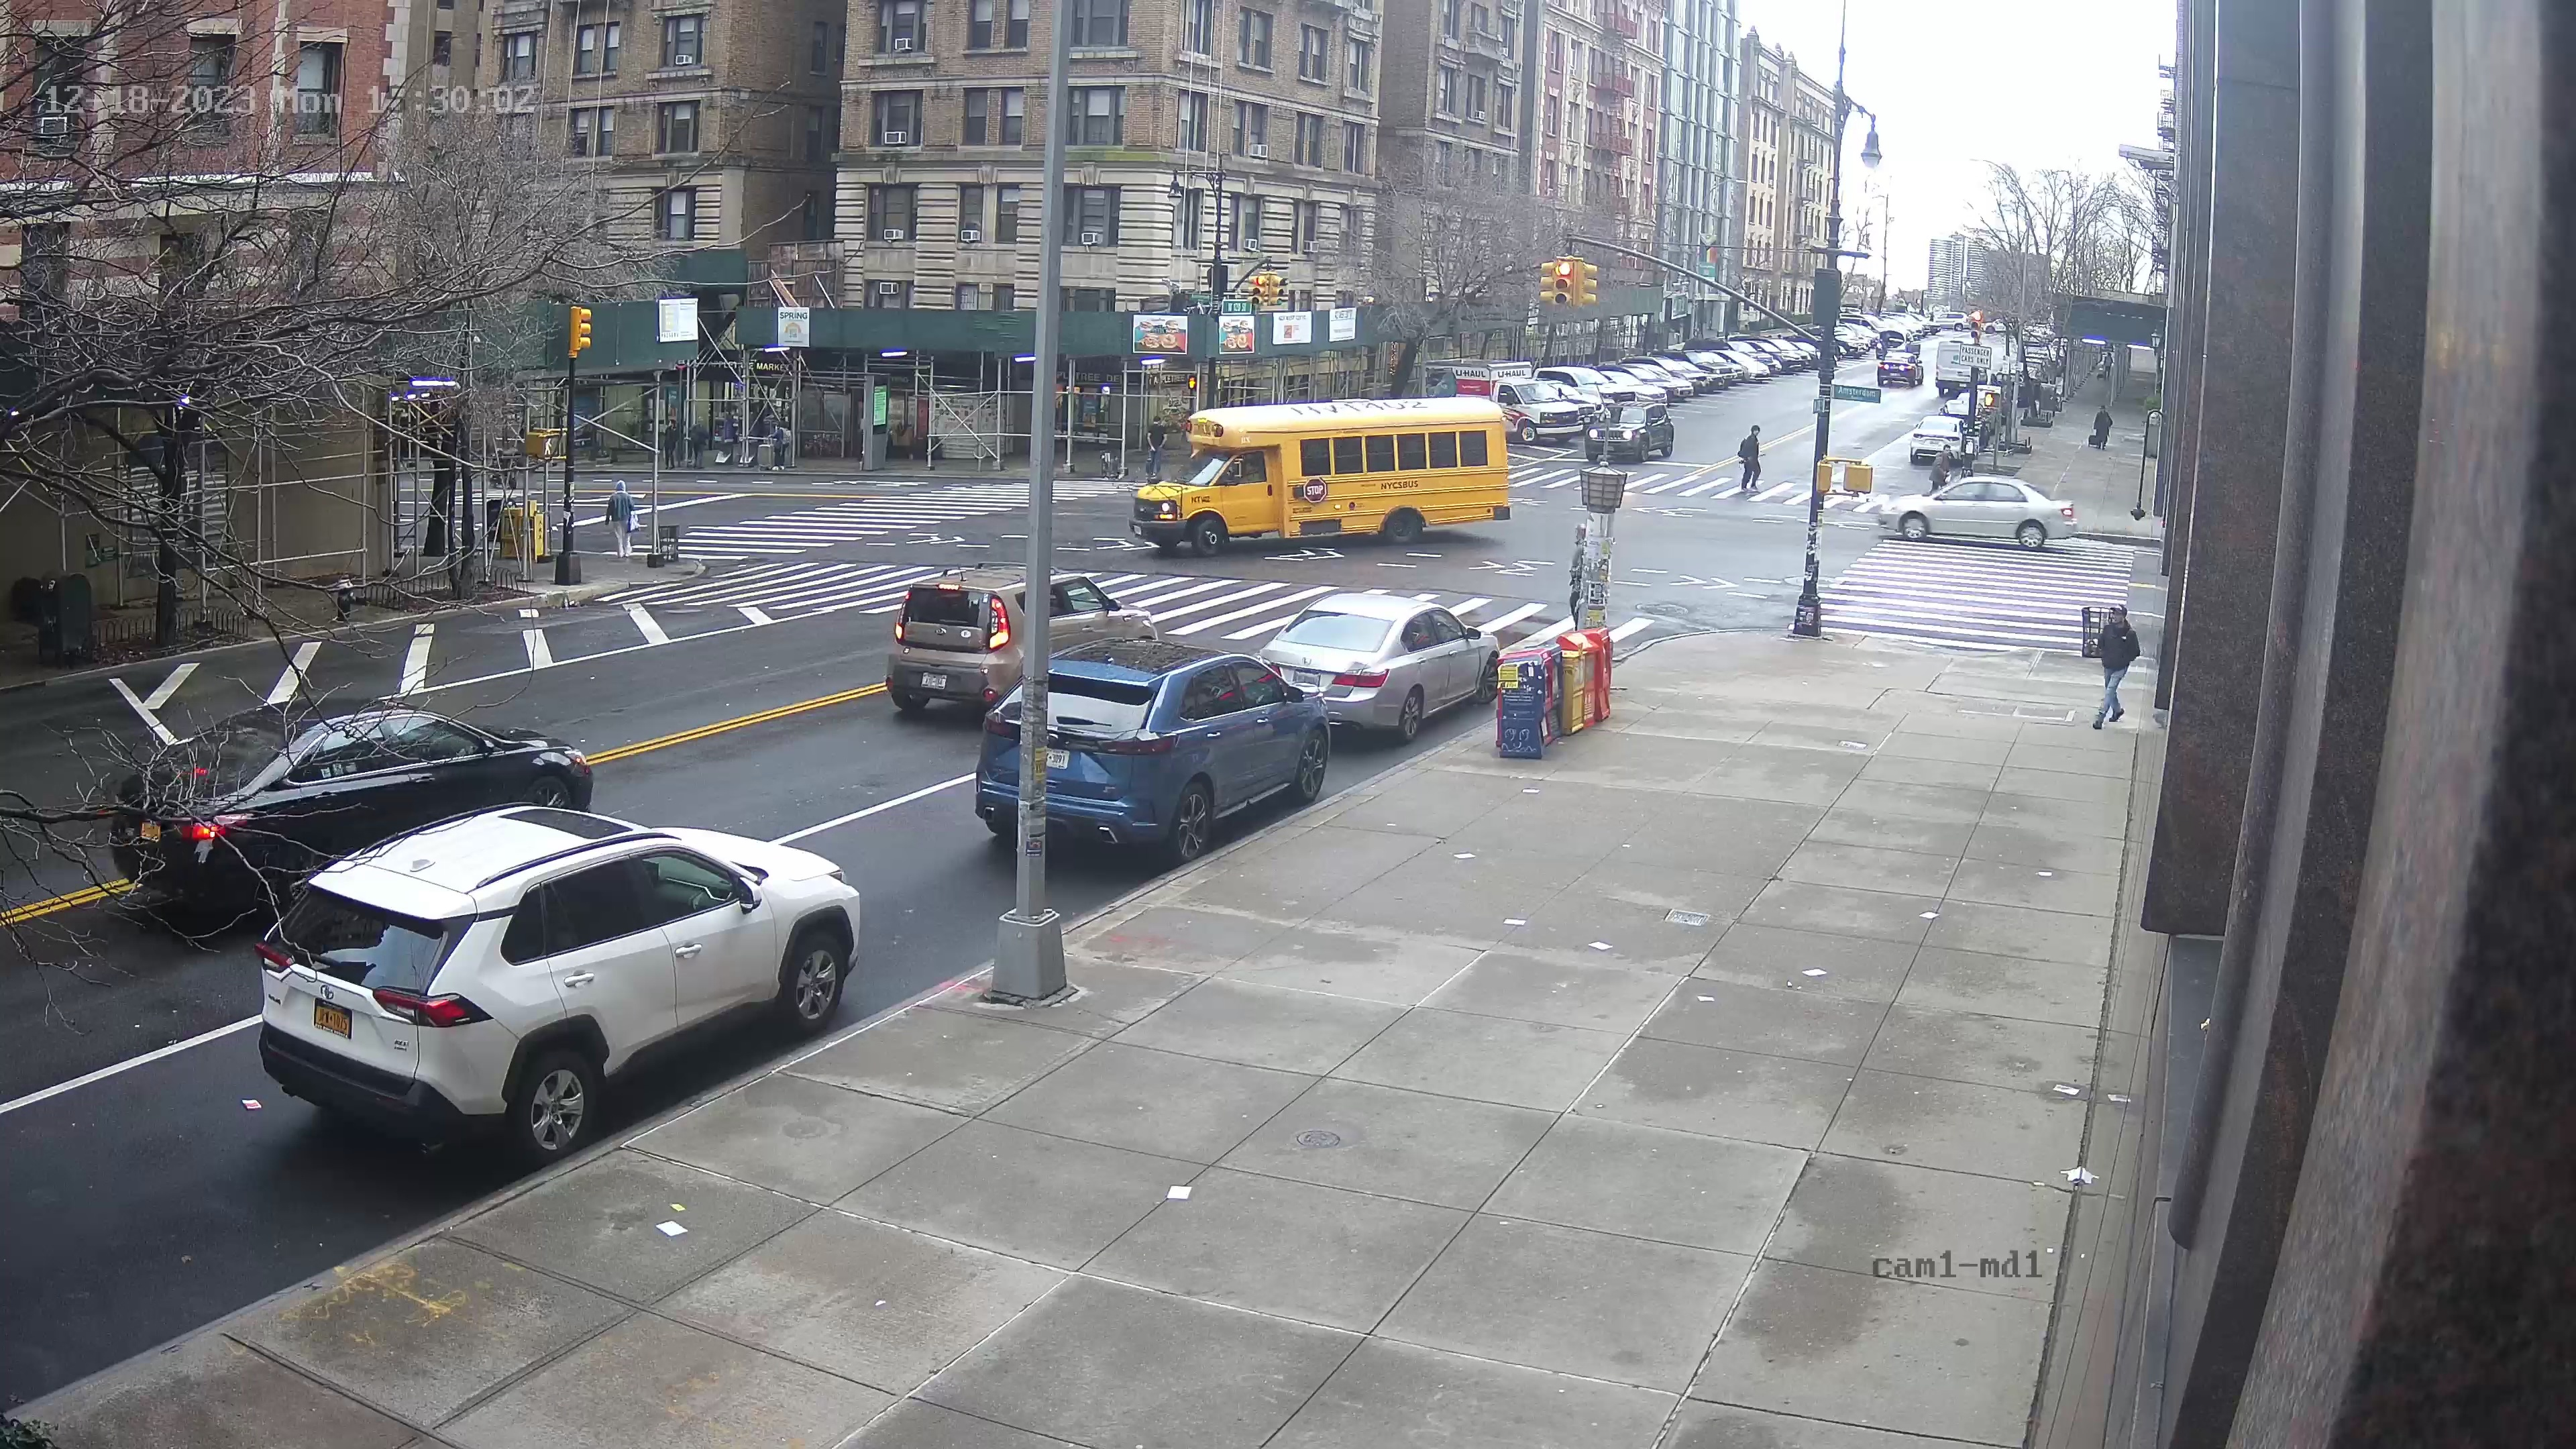
\includegraphics[width=8cm,height=8cm]{input.png}};

\pic[shift={(0,0,0)}] at (0,0,0) 
    {Box={
        name=conv1,
        caption= ,
        xlabel={{64, }},
        zlabel=224,
        fill=\ConvColor,
        height=64,
        width=2,
        depth=64
        }
    };

\pic[shift={ (0,0,0) }] at (conv1-east) 
    {Box={
        name=pool1,
        caption= ,
        fill=\PoolColor,
        opacity=0.5,
        height=32,
        width=1,
        depth=32
        }
    };

\pic[shift={(1,0,0)}] at (pool1-east) 
    {Box={
        name=conv2,
        caption= ,
        xlabel={{128, }},
        zlabel=112,
        fill=\ConvColor,
        height=32,
        width=2,
        depth=32
        }
    };

\pic[shift={ (0,0,0) }] at (conv2-east) 
    {Box={
        name=pool2,
        caption= ,
        fill=\PoolColor,
        opacity=0.5,
        height=32,
        width=1,
        depth=32
        }
    };

\pic[shift={(1,0,0)}] at (pool2-east) 
    {Box={
        name=conv3,
        caption= ,
        xlabel={{128, }},
        zlabel=56,
        fill=\ConvColor,
        height=25,
        width=2,
        depth=25
        }
    };

\pic[shift={ (0,0,0) }] at (conv3-east) 
    {Box={
        name=pool3,
        caption= ,
        fill=\PoolColor,
        opacity=0.5,
        height=32,
        width=1,
        depth=32
        }
    };

\pic[shift={(2,0,0)}] at (pool3-east) 
    {Box={
        name=fc1,
        caption=FC 512,
        zlabel=512,
        fill=\SoftmaxColor,
        height=25,
        width=1,
        depth=25
        }
    };

\pic[shift={(2,0,0)}] at (fc1-east) 
    {Box={
        name=fc2,
        caption=FC 4096,
        zlabel=4096,
        fill=\SoftmaxColor,
        height=25,
        width=1,
        depth=25
        }
    };

\pic[shift={ (1,0,0) }] at (fc2-east) 
    {Box={
        name=unpool1,
        caption= ,
        fill=\UnpoolColor,
        opacity=0.5,
        height=32,
        width=1,
        depth=32
        }
    };

\pic[shift={(0,0,0)}] at (unpool1-east) 
    {Box={
        name=uconv1,
        caption= ,
        xlabel={{32, }},
        zlabel=16,
        fill=\ConvColor,
        height=16,
        width=2,
        depth=16
        }
    };

\pic[shift={ (1,0,0) }] at (uconv1-east) 
    {Box={
        name=unpool2,
        caption= ,
        fill=\UnpoolColor,
        opacity=0.5,
        height=32,
        width=1,
        depth=32
        }
    };

\pic[shift={(0,0,0)}] at (unpool2-east) 
    {Box={
        name=uconv2,
        caption= ,
        xlabel={{64, }},
        zlabel=32,
        fill=\ConvColor,
        height=32,
        width=2,
        depth=32
        }
    };

\pic[shift={ (1,0,0) }] at (uconv2-east) 
    {Box={
        name=unpool3,
        caption= ,
        fill=\UnpoolColor,
        opacity=0.5,
        height=32,
        width=1,
        depth=32
        }
    };

\pic[shift={(0,0,0)}] at (unpool3-east) 
    {Box={
        name=uconv3,
        caption= ,
        xlabel={{128, }},
        zlabel=64,
        fill=\ConvColor,
        height=64,
        width=2,
        depth=64
        }
    };

\pic[shift={ (1,0,0) }] at (uconv3-east) 
    {Box={
        name=unpool4,
        caption= ,
        fill=\UnpoolColor,
        opacity=0.5,
        height=32,
        width=1,
        depth=32
        }
    };

\pic[shift={(0,0,0)}] at (unpool4-east) 
    {Box={
        name=uconv4,
        caption= ,
        xlabel={{128, }},
        zlabel=128,
        fill=\ConvColor,
        height=128,
        width=2,
        depth=128
        }
    };

\pic[shift={(1,0,0)}] at (uconv4-east) 
    {Box={
        name=uconv6,
        caption= ,
        xlabel={{4, }},
        zlabel=128,
        fill=\ConvColor,
        height=128,
        width=2,
        depth=128
        }
    };

\pic[shift={(1,0,0)}] at (uconv6-east) 
    {Box={
        name=output,
        caption= ,
        zlabel=4,
        fill=\SoftmaxColor,
        height=40,
        width=1,
        depth=40
        }
    };

\end{tikzpicture}
\end{document}
